\section{Results and Analysis}


\subsection{RQ1: Generalisation of FOLTR-ES performance beyond MQ2007/2008}
For answering RQ1 we replicate the results obtained by Kharitonov~\cite{kharitonov2019federated} on the MQ2007 and MQ2008 datasets; we then reproduce the experiment on MSLR-WEB10K and Yahoo datasets, on which FOLTR-ES has not been yet investigated, and we compare the findings across datasets. For these experiments we use antithetic variates, set $B = 4$ and 2,000 clients, use MaxRR as reward signal and for evaluation on clicked items. 

\begin{figure}[t]
	\centering
	\begin{subfigure}{1\textwidth}
		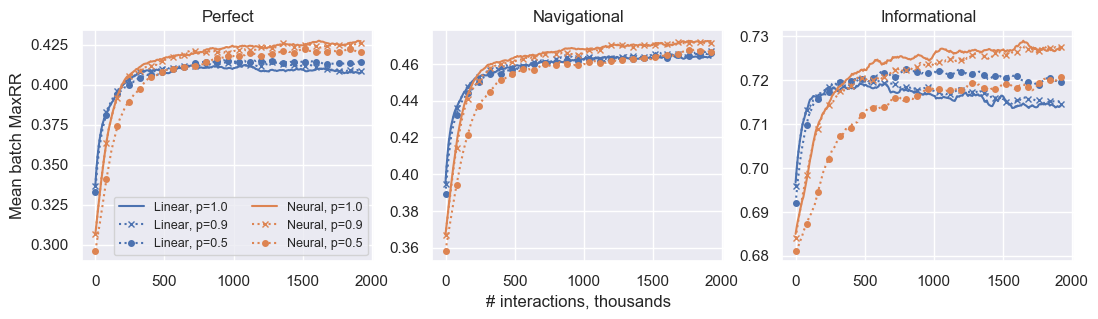
\includegraphics[width=15cm, height=3.5cm]{images/RQ1/mq2007_foltr_c2000_ps.png}
		\caption{Mean batch MaxRR for MQ2007.}
		\label{fig:mq2007-rq1}
	\end{subfigure}
	\begin{subfigure}{1\textwidth}
		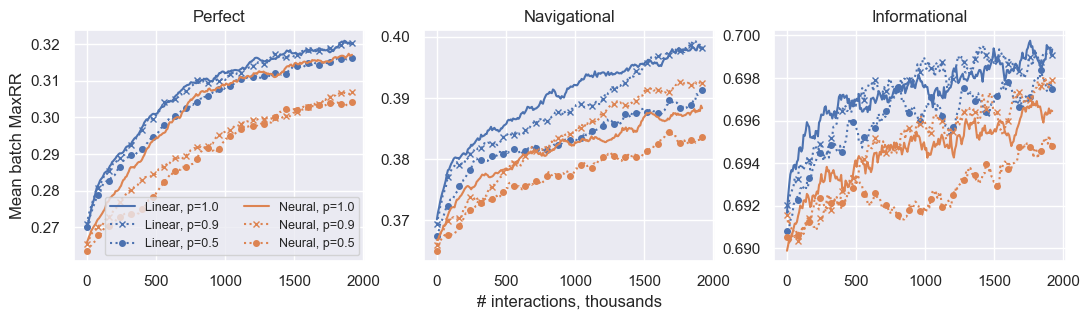
\includegraphics[width=15cm, height=3.5cm]{images/RQ1/mslr10k_foltr_c2000_ps.png}
		\caption{Mean batch MaxRR for MSLR10k}
		\label{fig:mslr10k-rq1}
	\end{subfigure}
	\begin{subfigure}{1\textwidth}
		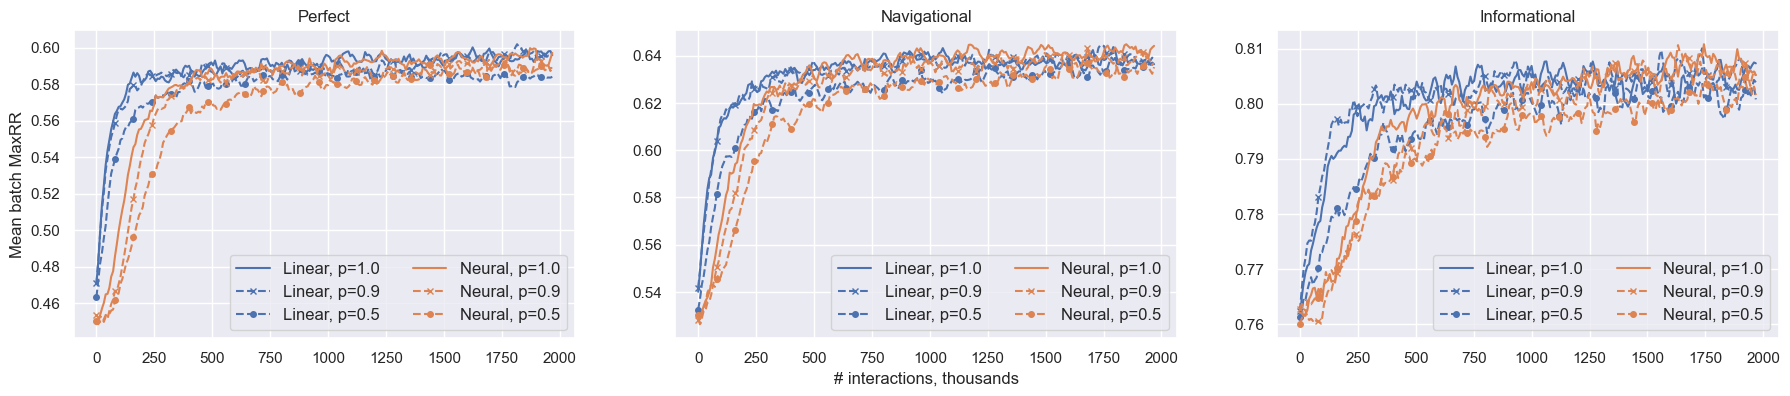
\includegraphics[width=15cm, height=3.5cm]{images/RQ1/yahoo_foltr_c2000_ps.png}
		\caption{Mean batch MaxRR for Yahoo.}
		\label{fig:yahoo-rq1}
	\end{subfigure}
	\caption{Results for RQ1: performance of FOLTR-ES across datasets. \label{fig:RQ1}}
\end{figure}

Figure~\ref{fig:mq2007-rq1} reports the results obtained by FOLTR-ES on the MQ2007 dataset\footnote{Similar results were obtained for MQ2008 and are omitted for space reasons.} with respect to the three click models considered, various settings for the privacy preservation parameter $p$, and the two FOLTR-ES methods (linear and neural). Our results fully replicate those of Kharitonov~\cite{kharitonov2019federated} and indicate the following findings: (1) FOLTR-ES allows for the iterative learning of effective rankers; (2) high values of $p$ (lesser privacy) provide higher effectiveness; 
(3) the neural ranker is more effective than the linear ranker when $p \rightarrow 1$ (small to no privacy), while the linear model is equivalent, or better (for informational clicks) when $p=0.5$. 

However, not all these findings are applicable to the results obtained when considering MSLR-WEB10K and Yahoo!, which are displayed in Figures~\ref{fig:mslr10k-rq1} and~\ref{fig:yahoo-rq1}. In particular, we observe that (1) the results for MSLR-WEB10K (and to a lesser extent also for Yahoo) obtained with the informational click model are very unstable, and, regardless of the click model, FOLTR-ES requires more data than with MQ2007/2008 to arrive at a stable performance, when it does; (2) the neural ranker is less effective than the linear ranker, especially on MSLR-WEB10K. We believe these findings are due to the fact that query-document pairs in MSLR-WEB10K and Yahoo! are represented by a larger number of features than in MQ2007/2008. Thus, more data is required for effective training, especially for the neural model; we also note that FOLTR-ES is largely affected by noisy clicks in MSLR-WEB10K. 

%In the previous work, FOLtR-ES is conducted on MQ2007 and MQ2008 datasets~\cite{kharitonov2019federated}. To further study if the algorithm can achieve similar ranking performance on other publicly available LTR datasets. We perform experiments on MSLR-WEB10K dataset using same parameters chosen by~\cite{kharitonov2019federated}, using antithetic variates and setting $B = 4$. 

%Unlike MQ2007 and MQ2008 datasets, FOLtR-ES performed on MSLR-WEB10K shows an opposite finding: the neural ranker dose not consistently perform better that the linear ranker. And for MSLR-WEB10K, FOLtR-ES takes more times on updating the ranker till it achieves the stable performance, which might be caused by larger training queries in MSLR-WEB10K. Figure \ref{fig: mq2007-rq1-1.0}\ref{fig: mslr-rq1-1.0}\ref{fig: mq2007-rq1-0.5}\ref{fig: mslr-rq1-0.5} show the mean batch MaxRR averaged on five data splits in MQ2007 and MSLR-WEB10K with the three click models.




%(Figures lack legend)
%\begin{figure}[H]
%	\centering
%	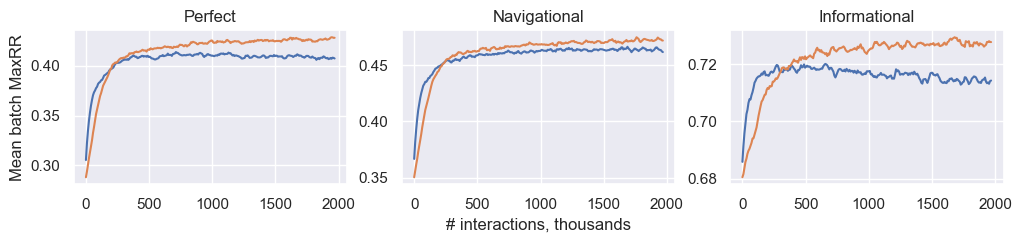
\includegraphics[width=15cm, height=3.5cm]{mq2007_foltr_c2000_p1.0.png}
%	\caption{Mean batch MaxRR for MQ2007 (2000 clients and $p = 0.9$)}
%	\label{fig: mq2007-rq1-1.0}
%\end{figure}
%\begin{figure}[H]
%	\centering
%	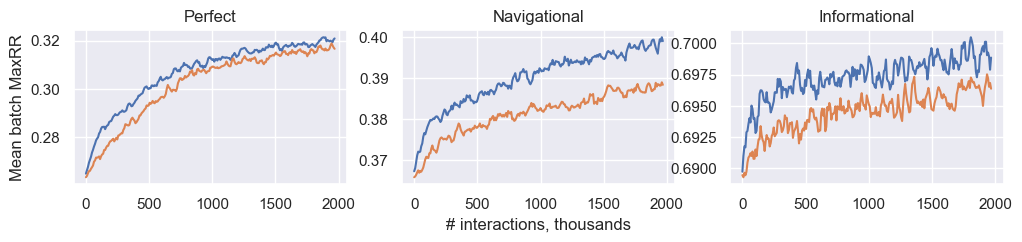
\includegraphics[width=15cm, height=3.5cm]{mslr10k_foltr_c2000_p1.0.png}
%	\caption{Mean batch MaxRR for MSLR-WEB10K (2000 clients and $p = 0.9$)}
%	\label{fig: mslr-rq1-1.0}
%\end{figure}
%
%\begin{figure}[H]
%	\centering
%	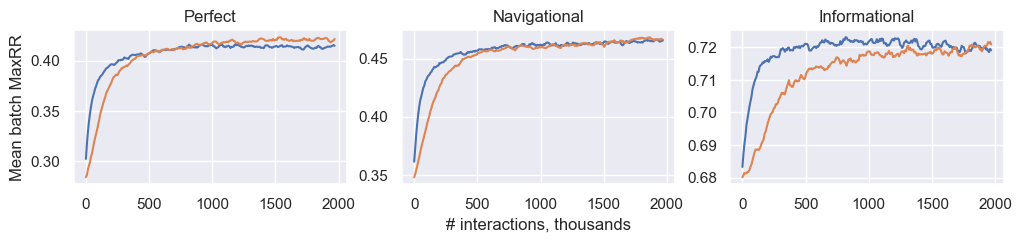
\includegraphics[width=15cm, height=3.5cm]{mq2007_foltr_c2000_p0.5.png}
%	\caption{Mean batch MaxRR for MQ2007 (2000 clients and $p = 0.5$)}
%	\label{fig: mq2007-rq1-0.5}
%\end{figure}
%\begin{figure}[H]
%	\centering
%	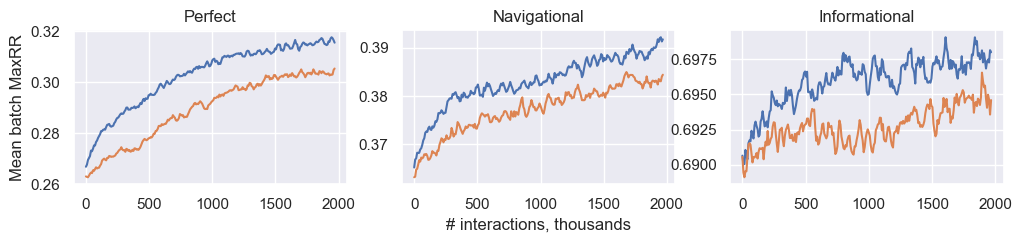
\includegraphics[width=15cm, height=3.5cm]{mslr10k_foltr_c2000_p0.5.png}
%	\caption{Mean batch MaxRR for MSLR-WEB10K (2000 clients and $p = 0.5$)}
%	\label{fig: mslr-rq1-0.5}
%\end{figure}

\subsection{RQ2: Effect of number of clients on FOLTR-ES}
%To answer RQ1, we perform experiments on MSLR-WEB10K dataset with the same FOLtR-ES setup
%Reproducing FOLtR-ES on other datasets

To answer RQ2 we vary thee number of clients involved in FOLTR-ES; we investigate the values \{50, 1,000, 2,000\}. Kharitonov~\cite{kharitonov2019federated} used 2,000 in the original experiments, and the impact of the number . To be able to fairly compare results across number of clients, we fixed the total number of ranker updates to 2,000,000; we also set $B = 4$ and set the privatization parameter $p=0.9$. We perform these experiments on all three datasets considered in this paper, but we omit to report results for Yahoo! due to space limitations. 


\begin{figure}[t]
	\centering
	\begin{subfigure}{1\textwidth}
		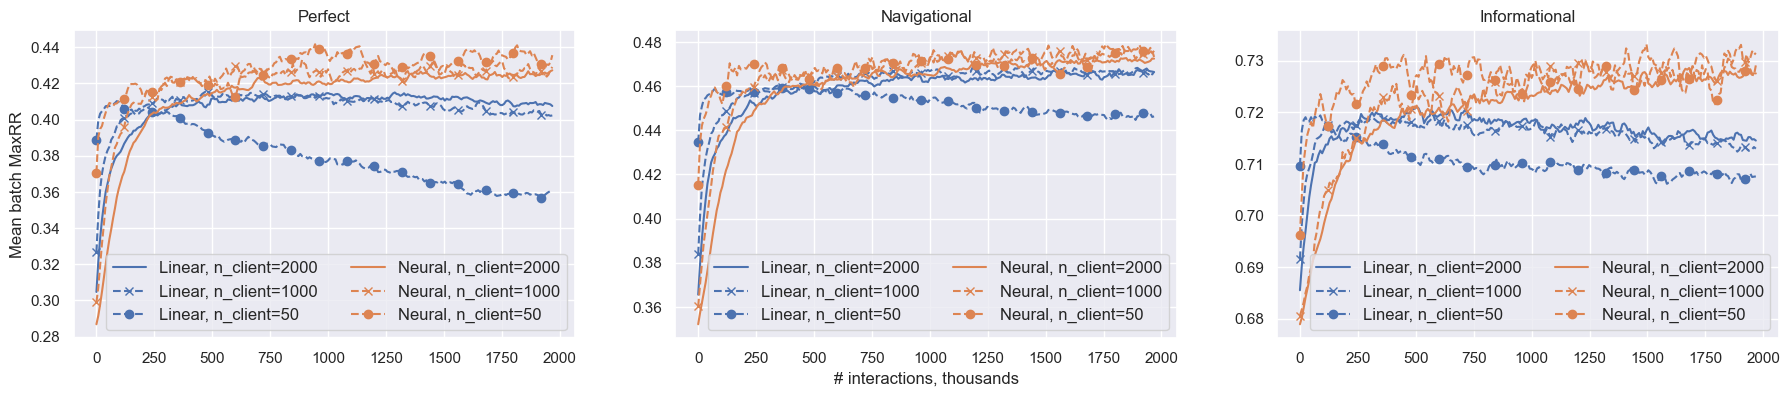
\includegraphics[width=15cm, height=3.5cm]{images/RQ2/mq2007_foltr_client_both_p0.9.png}
		\caption{Mean batch MaxRR for MQ2007.}
		\label{fig:mq2007-rq2}
	\end{subfigure}
	\begin{subfigure}{1\textwidth}
		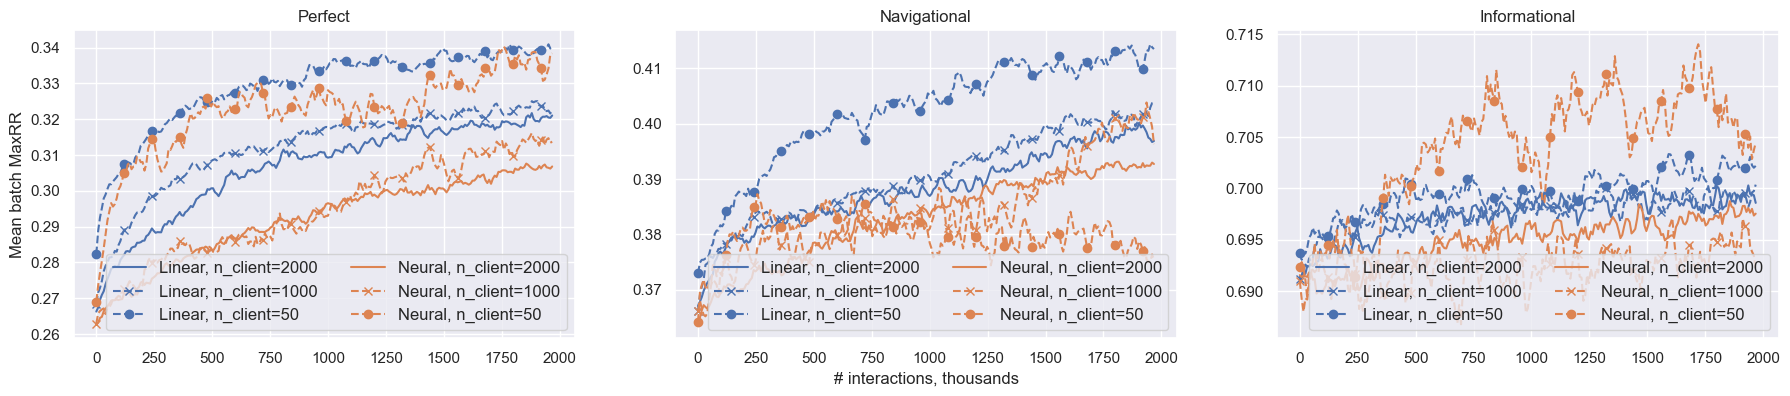
\includegraphics[width=15cm, height=3.5cm]{images/RQ2/mslr10k_foltr_client_both_p0.9.png}
		\caption{Mean batch MaxRR for MSLR10k}
		\label{fig:mslr10k-rq2}
	\end{subfigure}
	\caption{Results for RQ2: performance of FOLTR-ES with respect to number of clients. \label{fig:RQ2}} 
\end{figure}


The results of these experiments are reported in Figure~\ref{fig:RQ2}, and they are mixed. For MQ2007, the number of clients have little effect on the neural ranker used in FOLTR-ES, although when informational clicks are provided this ranker is less stable, although often more effective, if very few clients (50) are used. Having just 50 clients, instead, severally hits the performance of the linear ranker, when compared with 1,000 or 2,000 clients. The findings on MSLR10k, however, are different. In this dataset, a smaller number of clients (50), is generally better than larger numbers, both for linear and neural ranker. An exception to this is when considering navigational clicks: in this case the linear ranker obtains by far thee best performance with a small number of clients, but the neural ranker obtains the worst performance. This suggest that the number of clients greatly affects FOLTR-ES: but trends are not consistent across click types and datasets. 


%To study the influence of number of clients, we perform experiments on MQ2007 and MSLR-WEB10K datasets. We vary the number of clients across \{50, 1000, 2000\} but set the fixed total updating times to 2000000 and set $B = 4$. We also set the privatization parameter $p$ across \{0.5, 0.9, 1.0\}.

%Our experiments show that little clients number will reduce the performance in the linear ranker. But for the neural ranker, the difference is minor.

%\begin{figure}[H]
%	\centering
%	\includegraphics[width=16cm, height=8cm]{v0_mq2007_foltr_clients_p09.png}
%	\caption{Mean batch MaxRR for MQ2007 with different client number}
%	\label{fig: mq2007clients}
%\end{figure}
%\begin{figure}[H]
%	\centering
%	\includegraphics[width=15cm, height=3.5cm]{mq2007_foltr_client_linear_p09.png}
%	\caption{Mean batch MaxRR for MQ2007 with different client number (linear ranker and $p = 0.9$)}
%	\label{fig: mq2007-rq2-0.9}
%\end{figure}

\subsection{RQ3: Comparing FOLTR-ES to state-of-the-art OLTR methods}
The original study of FOLTR-ES did not compared the method with non-federated OLTR approaches. To contextualise the performance of FOLTR-ES and to understand the trade-off between privacy and performance done when designing FOLTR-ES, we compare this method with the current state-of-the-art OLTR method, the Pairwise Differentiable Gradient Descent (PDGD)~\cite{oosterhuis2018differentiable}. For fair comparison, we set the privatization parameter $p=1$ (lowest privacy) and the number of clients to 2,000. In addition note that in normal OLTR settings, rankers are updated after each user interaction: however in FOLTR-ES, rankers are updated in small batches. For fair comparison, we adapt PDGD to be updated in batch too. Instead of updating the ranker after each interaction (batch size 1), we accumulate gradients computed on the same batch size as for FOLTR-ES. Specifically, with 2000 clients for FOLTR-ES, the batch size of each update is 8,000 iterations (4 x 2,000). We then compute the updated gradients for PDGD on 8,000 interactions too. %Note, the number of updates after 2m user interaction now becomes 2m/8000 = 250.
We perform these experiments on all three datasets considered in this paper, but we omit to report results for Yahoo! due to space limitations. 

\begin{figure}[t]
	\centering
	\begin{subfigure}{1\textwidth}
		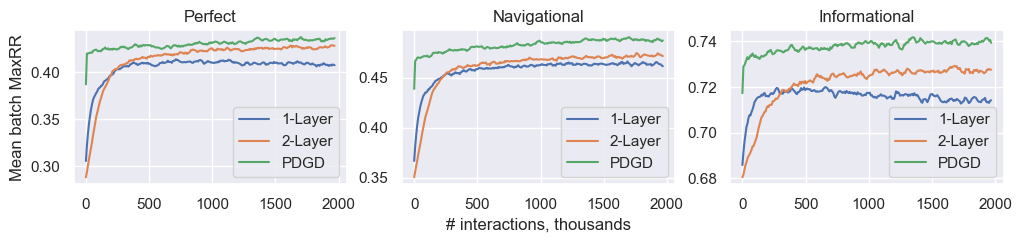
\includegraphics[width=15cm, height=3.5cm]{images/RQ3n4/mq2007_foltr_PDGD_mrr_c2000_p1.0}
		\caption{Mean batch MaxRR for MQ2007.}
		\label{fig:mq2007-rq3}
	\end{subfigure}
	\begin{subfigure}{1\textwidth}
		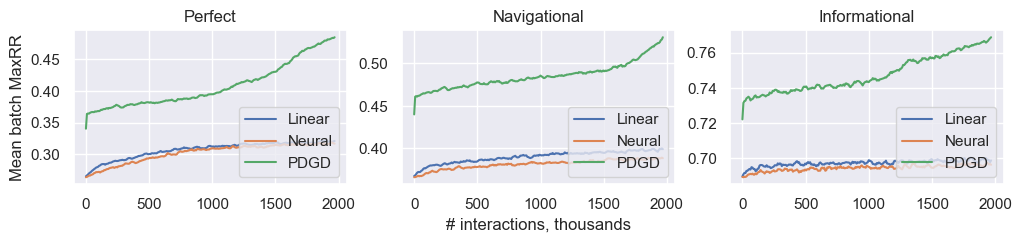
\includegraphics[width=15cm, height=3.5cm]{images/RQ3n4/mslr10k_foltr_PDGD_mrr_c2000_p1.0.png}
		\caption{Mean batch MaxRR for MSLR10k}
		\label{fig:mslr10k-rq3}
	\end{subfigure}
	\caption{Results for RQ3: performance of FOLTR-ES and PDGD across datasets. \label{fig:RQ3}} 
\end{figure}

Results are shown in Figure~\ref{fig:RQ3}: regardless of linear or neural ranker, FOLTR-ES is less effective than PDGD. The gap in performance is greater in larger datasets like MSLR10k and Yahoo! (not shown) than in the smaller MQ2007/2008. This gap becomes even bigger, especially for the first iterations, if the PDGD ranker was updated after each iteration (not shown here), rather than after a batch has been completed. This highlights that FOLTR-ES has the merit of being the first privacy preserving federated OLTR approach available; however, more work is needed to improve the performance of FOLTR based methods so as to close the gap between privacy-oriented approaches and centralise approaches that do not consider user privacy.

%In order to further study the ranking quality, especially users' experience in FOLtR-ES, we perform experiments on comparing FOLtR-ES with the current state-of-the-art OLTR methods. In this section, we choose Pairwise Differentiable Gradient Descent (PDGD) models as baselines. For a fair comparation, we set up the privacy probability $p = 1$ (lowest privacy) in FOLtR-ES. We perform experiments on MQ2007 and MSLR-WEB10K datasets with simulating 2000 clients.

%Based on the experiment results, we can see FOLtR-ES still lags behind OLTR methods in terms of the ranking performance. As the ranking quality is an essential metric for web search engines, future work can be extend to improving ranking performance and in the meantime, protecting users' privacy.

%\begin{figure}[H]
%	\centering
%	\includegraphics[width=16cm, height=8cm]{v0_mq2007_foltr_vs_pdgd_2000clients_p10.png}
%	\caption{Mean batch MaxRR for MQ2007 with 2000 clients and $p = 1$}
%	\label{fig: mq2007-v0-baseline}
%\end{figure}
%
%\begin{figure}[H]
%	\centering
%	\includegraphics[width=16cm, height=8cm]{v0_mslr_foltr_vs_pdgd_2000clients_p10.png}
%	\caption{Mean batch MaxRR for MSLR-WEB10K with 2000 clients and $p = 1$}
%	\label{fig: mslr-v0-baseline}
%\end{figure}
%
%\begin{figure}[H]
%	\centering
%	\includegraphics[width=15cm, height=3.5cm]{mq2007_foltr_PDGD_mrr_c2000_p10.png}
%	\caption{Mean batch MaxRR for MQ2007 with two FOLtR-ES ranker(2000 clients and $p = 1$) and PDGD baselines}
%	\label{fig: mq2007-rq3}
%\end{figure}


\subsection{RQ4: Extending FOLTR-ES evaluation to common OLTR practice}

In the original work and in the sections above, FOLTR-ES was evaluated using MaxRR computed with respect to the clicks performed by the simulated users (click models). This is an unusual evaluation for OLTR because: (1) usually nDCG@10 is used in place of MaxRR as metric, (2) nDCG is computed with respect to relevance labels, and not clicks, and on a withheld portion of the dataset, not on the interactions observed -- this is used to produce learning curves and is referred to as offline nDCG, (3) in addition online nDCG is measured from the relevance labels in the SERPs from which clicks are obtained, and either displayed as learning curves or accumulated throughout the sessions -- these values represent how OLTR has affected user experience. We then consider this more common evaluation of OLTR next, where we set the number of clients to 2,000 and experiment with $p=\{0.5, 0.9, 1.0\}$; we omit to report results for Yahoo! due to space limitations. 


\begin{figure}[t]
	\centering
	\begin{subfigure}{1\textwidth}
		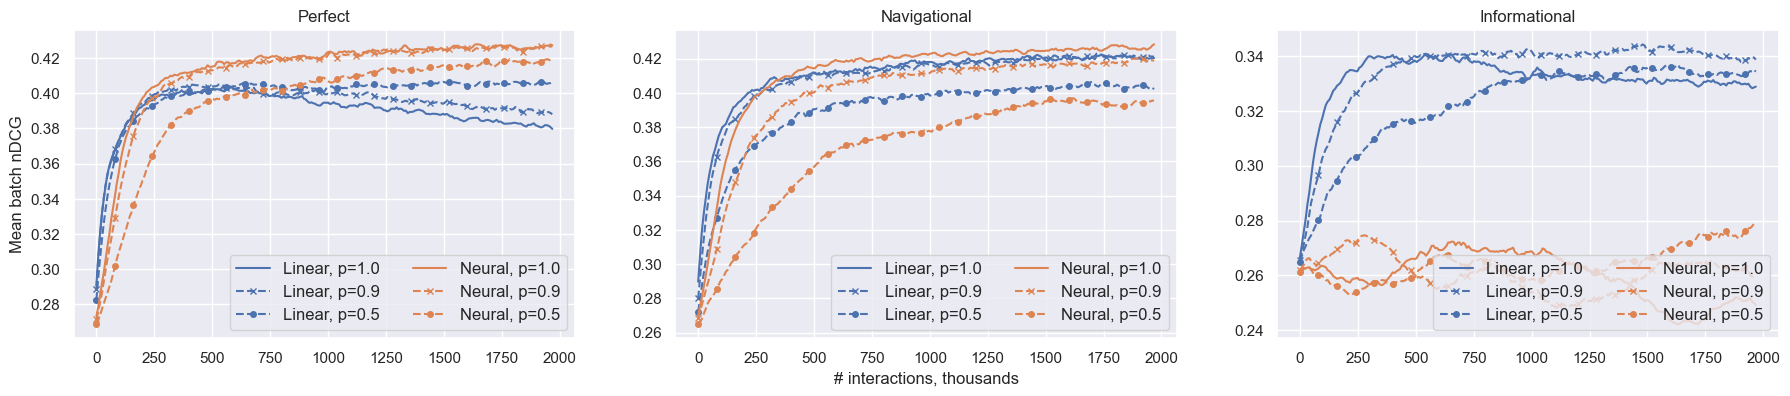
\includegraphics[width=15cm, height=3.5cm]{images/RQ3n4/mq2007_foltr_DCG_both_c2000_ps.png}
		\caption{Mean batch nDCG@10 for MQ2007.}
		\label{fig:mq2007-rq4}
	\end{subfigure}
	\begin{subfigure}{1\textwidth}
		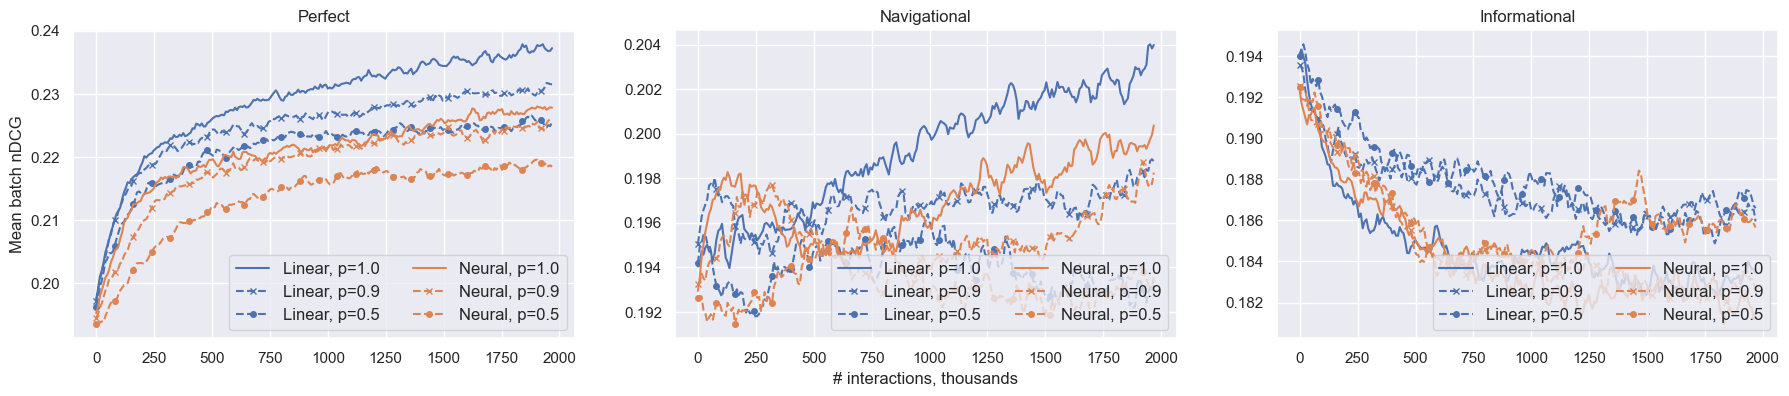
\includegraphics[width=15cm, height=3.5cm]{images/RQ3n4/mslr10k_foltr_DCG_both_c2000_ps.png}
		\caption{Mean batch nDCG@10 for MSLR10k.}
		\label{fig:mslr10k-rq4}
	\end{subfigure}
	\caption{Results for RQ4: performance of FOLTR-ES in terms of online nDCG@10 computed using relevance labels and the SERPs used for obtaining user iterations. \label{fig:RQ4}} 
\end{figure}

\begin{figure}[t]
	\centering
	\begin{subfigure}{1\textwidth}
		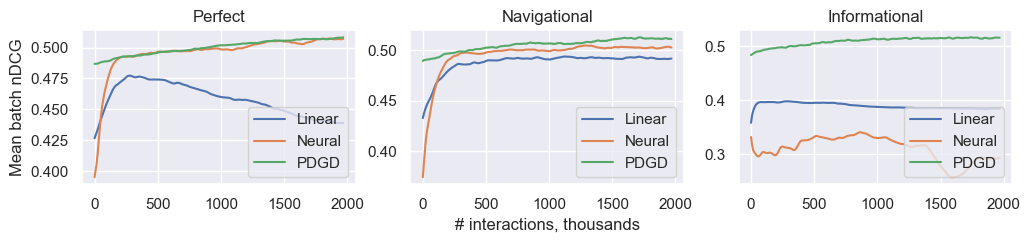
\includegraphics[width=15cm, height=3.5cm]{images/RQ3n4/mq2007_foltr_PDGD_offline_ndcg_c2000_p1.0.png}
		\caption{Mean batch nDCG@10 for MQ2007.}
		\label{fig:mq2007-rq4-offline}
	\end{subfigure}
	\begin{subfigure}{1\textwidth}
		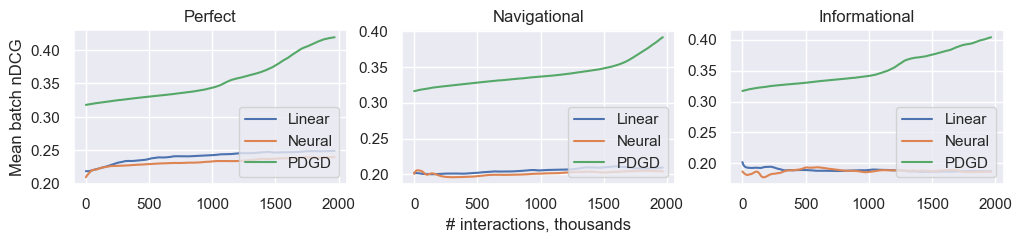
\includegraphics[width=15cm, height=3.5cm]{images/RQ3n4/mslr10k_foltr_PDGD_offline_ndcg_c2000_p1.0.png}
		\caption{Mean batch nDCG@10 for MSLR10k.}
		\label{fig:mslr10k-rq4-offline}
	\end{subfigure}
	\caption{Results for RQ4: performance of FOLTR-ES and PDGD in terms of offline nDCG@10. \label{fig:RQ4-offline}} 
\end{figure}

Results are reported in Figure~\ref{fig:RQ4}. It is interesting to compare these plots with those in Figure~\ref{fig:RQ1}, that relate to the unusual (for OLTR) evaluation setting used in the original FOLTR-ES work. By comparing the figures, we note that for MQ2007, FOLTR-ES can effectively learn rankers for perfect and navigational clicks. However, when the clicks become nosier (informational clicks), then FOLTR-ES learning is effective for the linear ranker but no learning occurs for the neural ranker: this is unlikely in the evaluation settings of the original work (Figure~\ref{fig:RQ1}). We note this finding repeating also for MSLR10k, but this time this affects both linear and neural rankers; we also note that the online performance in MSLR10k on navigational clicks are also quite unstable and exhibit little learning for specific values of $p$ and ranker type. 


We further investigate the performance of FOLTR-ES with respect to offline nDCG@10. Results are shown in Figure~\ref{fig:RQ4-offline}, and are plotted along with the offline nDCG@10 of PDGD for additional context. Also the offline performance confirm that FOLTR-ES does not provide stable learning across click settings, datasets and ranker types. We also note that the performance of PDGD are sensibly higher than that of FOLTR-ES, apart for the neural ranker on MQ2007 when perfect and navigational clicks are considered. 

These findings suggest that FOLTR-ES is yet far from being a solution that can be considered for use in practice, and more research is required for devising effective federated, privacy-aware OLTR techniques.


%To study the generalisation of FOLtR-ES to other common OLTR evaluation metrics, we use Discounted Cumulative Gain (DCG) to evaluate the users' experience in each interaction. We also compute NDCG@10 with the relevance labels to evaluate the central ranker with test data as we want to explore the stability of  performance in FOLtR-ES.

%In terms of nDCG evaluation, although FOLtR-ES achieves decent performance (with nDCG exceed 0.4 except for $Informational$ model), it still falls behind the PDGD baselines.

%\begin{figure}[H]
%	\centering
%	\includegraphics[width=15cm, height=3.5cm]{mq2007_foltr_PDGD_ndcg_c2000_p10.png}
%	\caption{Mean batch MaxRR for MQ2007 with(2000 clients and $p = 1$)}
%	\label{fig: mq2007-rq4}
%\end{figure}

